\section{Menusystem}\label{sec:menu}
For at kunne ændre på equalizerens parametre og indstillinger, skal der være en form for menusystem. Dette menusystem skal opbygges på en måde, så det ikke forstyrrer mikroprocessorens andre igangværende processer (såsom håndtering af lydsignalet som er den primære funktion). Derfor opsættes en buffer som kan modtage data når det bliver tilgængeligt, og når der er tid til at håndtere dette. Visning af menu på displayet og håndtering af de diverse inputs, skal foregå meget enkelt, da der i alt kun er 1024 clock cycles tilbage efter håndtering af lydsignalet. \\
\husk{Søren}{Skal evt. rettes til så det passer til shell}

\begin{figure}[h]
	\centering
	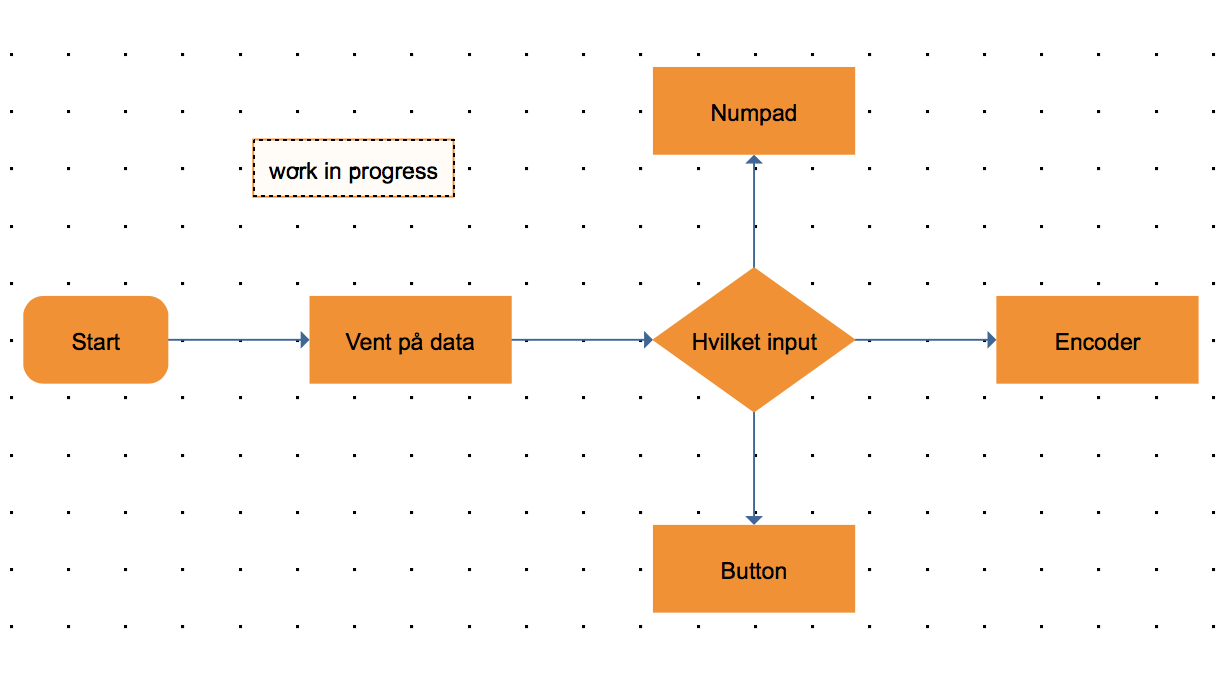
\includegraphics[width=15cm]{billeder/ui_flowchart}
	\caption{Menusystemets opbygning beskrevet med et flowchart. \husk{Søren}{WIP!}}
\end{figure}

Menusystemet sørger for at "lytte" efter eventuelt indkommende data, og skal, når der er data tilgængeligt, behandle den derefter. I denne buffer kan der være tre forskellige ting som har indflydelse på hvad der skal ske. Der er på "EMP-board"'et en numpad, dedikerede knapper, og en encoder. LCD'en er det hovedsagelige i UI'et, da det er her brugeren kan se hvor i menuen man er, samt se hvad indstillingerne er og hvad de eventuelt skal ændres til.

\section{I$^2$C}\label{sec:i2c}
For at implementere et kommunikationssystem til at styre equalizeren, bruges I$^2$C. På den måde kan en anden microcontroller kommunikere og ændre indstillinger og profiler. Da EMP-boardet ikke bruges, og der derfor ikke er noget LCD display, er dette umiddelbart den bedste løsning. På den måde tager vi også en del load af selve EQ-microkontrolleren, da User Interfacet foregår på en ekstern mikrokontroller.

Dette gør det også nemmere at senere tilføje moduler til User Interfacet, da I$^2$C protokollen allerede er trådt i kraft, og man kun behøver at ændre kode på den eksterne mikrokontroller.

\section{LCD}\label{sec:lcd}
LCD displayet viser equalizerens status informationer. Man kan se den igangværende eq-profil - altså hvilken lydindstilling der aktuelt kører. Derudover er der et VU-meter, som bliver brugt til at se om der er signal igennem, samt hvor højt det er. På den måde kan man se om den overstyrer. Til sidst er der en CPU-load indikator. Med denne indikator kan der afgøres om der er plads til at indsætte endnu et bånd på equalizeren. Problemet med sådan et LCD display, er at det tager for mange CPU-cycles at skrive til, så derfor er der implementeret en metode til at håndtere dette. \\

Da der som tidligere nævnt kun er $1814$ CPU-cycles mellem hver interrupt/sample, kan hele LCD'en ikke opdateres på en gang, da dette ville tage mere end $1814$ cycles. Derfor er der implementeret en buffer, hvor den skriver til ét felt på LCD'en, ved hver interrupt. Det tager ingen tid at skrive til denne buffer, så derfor spares der på CPU-cycles, så de kan bruges til noget der er vigtigere (f.eks. DSP). Da LCD'en så har sin egen task, kan den skrive hvad der ligger i bufferen når der er tid til det. \\

\subsection{Infodisplay}
LCD'et viser som tidligere nævnt forskellige informationer om equalizerens status, men da den også skal vise "grafik" i form at et VU-meter, skal det først sættes op korrekt. Da LCD-displayet normalt kun kan modtage ASCII\footnote{https://en.wikipedia.org/wiki/ASCII} tegn, er der opsat en custom "font", som gør at man kan udfylde alle pixels i et felt. På den måde kan der laves linjer/kasser, så man kan visualisere et VU-meter. (se kode)\\
 
\begin{figure}[h]
	\centering
	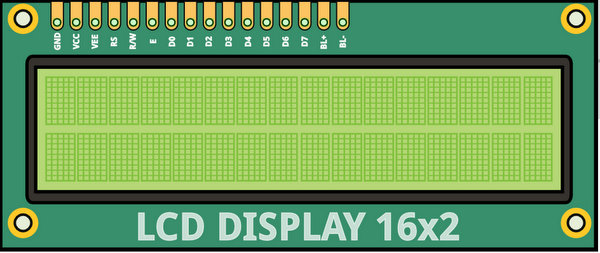
\includegraphics[width=7cm]{billeder/lcd_pixels}
	\caption{Eksempel på fyldt pixel/custom font}
\end{figure}

\husk{Søren}{Ændr' billede af pixels i VU}

Der vises også den igangværende profil som vælges vha. shell'en (se kapitel \ref{sec:shell}). På den måde giver det brugeren et feedback på at den valgte profil er trådt i kraft. 

Til sidst vises det aktuelle CPU-load, og denne procentdel udregnes ud fra de ledige clock cycles der er tilbage efter behandling af lyd. \husk{Søren}{Mere info om udregningen her}

\subsection{Initialisation}
LCD'et kræver en speciel rutine for at starte korrekt. LCD'en har forskellige muligheder som man kan sætte op, f.eks. en blinkende cursor, og om den automatisk skal gå til næste felt når den har skrevet i det nuværende. I dette tilfælde er den sat op, så der ikke er en blinkende cursor, og så den automatisk går til næste felt. Der skal også specificeres antallet af pixels, antallet af linjer samt hvilken font der skal bruges. Denne rutine kaldes i starten, så displayet er klar til brug når equalizeren starter. 

\section{Shell}\label{sec:shell}
For at brugeren kan ændre den valgte profil, er der implementeret et shell script, som tager imod korte kommandoer. Her kan man også aflæse hvilke tasks der kører, samt hvilken prioritet de har. For at kunne kommunikere med shell'en, skal UART'en sættes op, så man via en computer kan indtaste de forskellige kommandoer. 

\husk{Søren}{Billede af shell start/welcome}

I dette vindue sender man sine kommandoer 


